\documentclass[letterpaper,12pt]{article}
\usepackage{tabularx} % extra features for tabular environment
\usepackage{amsmath}  % improve math presentation
\usepackage{graphicx} % takes care of graphic including machinery
\usepackage[margin=1in,letterpaper]{geometry} % decreases margins
\usepackage{cite} % takes care of citations
\usepackage[final]{hyperref} % adds hyper links inside the generated pdf file
\hypersetup{
	colorlinks=true,       % false: boxed links; true: colored links
	linkcolor=blue,        % color of internal links
	citecolor=blue,        % color of links to bibliography
	filecolor=magenta,     % color of file links
	urlcolor=blue         
}
\usepackage{blindtext}
%++++++++++++++++++++++++++++++++++++++++


\begin{document}

\title{Web Application Security Threat - SQL injection}
\author{Anshumaan Singh 18BCE2193}
\date{\today}
\maketitle

\begin{abstract}
In this assignment paper we studied the concept of SQL injection which is a serious threat to Web Application Security. A brief research has been generated on it and it's preventive measures have been discussed and well versed for the readers.   
\end{abstract}


\section{Introduction}

With the spread of the Internet and the WEB's rapid development, WEB applications not only improved the efficiency of work and enterprise strengthens the enterprise market competitiveness. Web platform have flexible, efficient, low cost and other information superiority has greatly improved the related department work efficiency, and promote the actual business thorough development, enhance
the department and the outside world exchange, service and interaction. Our country's computer
industry after more than ten years of development, the national industry production management
system, are based on the Internet architecture, in the country's defense engineering, government office,
financial systems, to network games, online banking, network transactions, is inseparable from the
network. Today's Internet has become the indispensable part in life. How to effectively ensure network
stability and safety operation is an important topic, also is the various network managers have a
headache problem. 
Attack  SQL  injection  is  to  use  the  insert  harmful  character  attacktechnology.   The  attacker  using  programmers  to  user  input  data  legitimacy  detection  notstrictly or not detection characteristics,  deliberately in a different way from client submitspecial code to manipulate data, thus collection procedures and server information, obtainthe desired information.




\section{Background}

SQL Injection is an attack technique used to exploit applications that construct SQL statements from user-supplied input. When successful, the attacker is able to change the logic of SQL statements executed against the database.Due to the various Web server vulnerabilities and procedure of the rigor leads to a Web server script for attacks was increasing, its are mostly through the ASP or PHP scripting injection such as a major attack means, plus Web site rapid expansion of today, based on both the SQL injection also slowly become the mainstream way. Attack SQL injection is to use the insert harmful character attack technology. The attacker using programmers to user input data legitimacy detection not strictly or not detection characteristics, deliberately in a different way from client submit special code to manipulate data, thus collection procedures and server information, obtain the desired information.

\begin{figure}[!h]
    \centering
    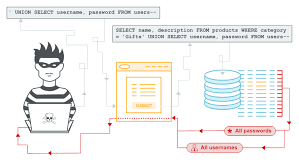
\includegraphics[width=.8\textwidth]{sqlinjection.png}
    \caption{SQL Injection is an attack technique used to exploit applications that construct SQL statements from user-supplied input.  When successful, the attacker is able to change the logicof SQL statements executed against the database.}
\end{figure}

\section{Web Security Situation}

With the deepening of the network applications, the Internet website quantity with amazing speed
increase. Whether government departments, enterprises and various management agencies, through the
website to establish various information platform for various business applications. Website is
information release center, its database to store has a large amount of for users to share the important
information and materials. Therefore, to ensure the normal operation of the web site, the security is
website construction and operation process should be fully considered important issues. Although the
Internet application scale developed rapidly, but the complexity of the network environment, and
information system, variability of vulnerability, decide the existing computer system still does not have
with own application development scale of corresponding security protection ability, a large number of
online threats USES all sorts of hidden way constantly pounding network application platform.
Network security problems are not reflected in the technical level of information counter, in actual
social activities, threat generated more from the huge interest drive. 
Internet is an open, no control agency network, based on TCP/IP protocol Internet protocol families
own open great place show various computer networking and interconnection and directly, and
promoted the rapid development of Internet technology. But as in the early network protocol design
neglect the safety, cause Internet in use and management of chaos, and gradually make the Internet
itself of safety and security has been threatened. Hackers (Hacker) often get the chance to intrude into
the computer on the network system, or stolen confidential data and theft privilege, or destroy the
important data, or make the system function not fully exert until paralysis.
Website unauthorized access to web security will be fatal, and its harm degree is the largest.
System password simple and short, operating system of various vulnerabilities, various applications
software defect, the default Shared folder, a large number of network application service of opening,
safety level set too low for hackers illegal invasion will offer a convenient. 
With the expanding of network size, computer network virus to site the threat of a bigger role. Network
virus spread on the Internet very fast, and its harm is enormous. 




\section{SQL injection}

Due to the various Web server vulnerabilities and procedure of the rigor leads to a Web server script for
attacks was increasing, its are mostly through the ASP or PHP scripting injection such as a major attack means,
plus Web site rapid expansion of today, based on both the SQL injection also slowly become the mainstream way.
Attack SQL injection is to use the insert harmful character attack technology. The attacker using programmers to
user input data legitimacy detection not strictly or not detection characteristics, deliberately in a different way from
client submit special code to manipulate data, thus collection procedures and server information, obtain the desired
information. This paper briefly introduces the concept of SOL injection attack and principle, and the realization
process of SQL injection attack, and on this basis describes how to detect SQL injection attack, summarizes the
general SQL injection attack prevention methods. And the ASP website platform system injection attack
prevention technology examples are analyzed, make prevent SQL injection technology in the practical application
of web security system plays a better, more effectively resist hackers and other malicious damage.

\begin{figure}[!h]
    \centering
    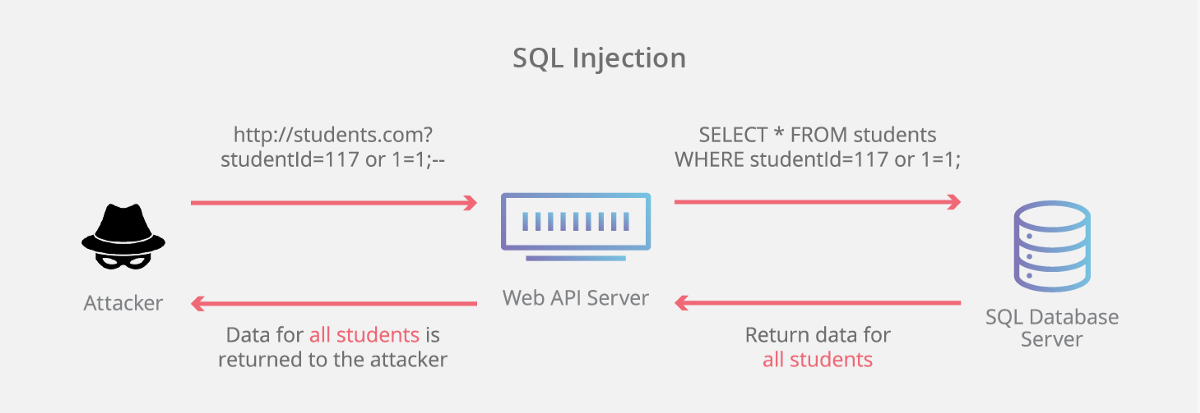
\includegraphics[width=.8\textwidth]{pic2.png}
    \caption{The attacker using programmers to userinput data legitimacy detection not strictly or not detection characteristics, deliberately in adifferent way from client submit special code to manipulate data, thus collection proceduresand server information,  obtain the desired information.}
\end{figure}

\section{Preventive Measures}

The use of parameterized lactobacillus colonisation statement
To defense SQL injection, user input is absolutely cannot directly to be embedded SQL statements.
On the contrary, the user input must be filtered, or use of parameterized statement. Parametric
statements and not use parameters user input into the statement. In most cases, the SQL statement was
fixed. Then, the user input will be limited to a parameter.
To avoid using explain program, because that's what hackers to perform an illegal means of
command.
Prevent SQL injection, and avoid some detailed error messages, because the hackers can use the
information. To use a standard input mechanism to verify all confirmed the input data of length, type, a
statement, enterprise rules, etc.
Using professional vulnerability scanning tools. 
\begin{figure}[!h]
    \centering
    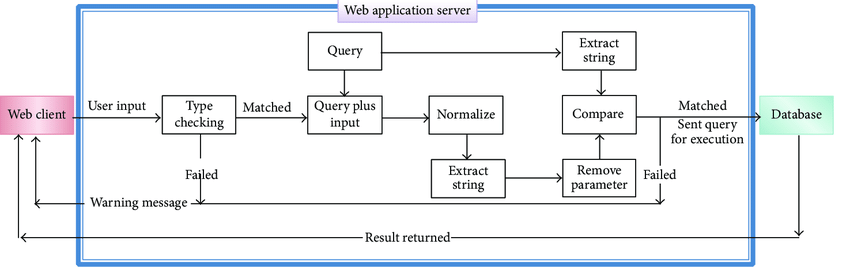
\includegraphics[width=.8\textwidth]{Model-for-prevention-of-SQL-injection-attack.png}
    \caption{The use of parameterized lactobacillus colonisation statement To defense SQL injection, userinput is absolutely cannot directly to be embedded SQL statements.}
\end{figure}




\section{Conclusions}
In this paper the SOL injection attack method, principle and attack implementation process is
discussed and summarized in this paper, due to a SQL injection attack is for application development
process of the programming loophole, so for the vast majority of firewall speaking, this kind of attack
can be bypassed. Although the database server version has been updated, various scripting language
itself fewer vulnerabilities, but as SOL injection technology unceasing enhancement, as long as the
Web application system or source still existed in such loophole, will lurk this concern, especially when
SOL injection attack with some other attack tool with, the server and system are huge threat.
Therefore, the study SQL injection attack prevention methods, pay attention to the safety of SOL
Server configuration, strengthening the code to user input information filtering check to develop safe
Web applications has important significance. With the development of network security technology,
also need to SQL injection attack technology to do further research, due to the SQL injection technique
quite flexible, in injection time will come across many unexpected situation. Therefore in setting up
Web server to overall consideration host and the security of the system, set up the server and the
database security options, completes the code's safety inspection work, so that we can do to prevent this,
the greatest degree realizes network security. 

\begin{table}[ht]
\begin{center}
\caption{Research Papers used extensively as base paper.}
\label{tbl:bins} % spaces are big no-no withing labels
\begin{tabular}{|cc|} 
\hline
\multicolumn{1}{|c}{$Paper$ } & \multicolumn{1}{c|}{$Publisher$ } \\
\hline
Review of SQL Injection : Problems and Prevention &   Researchgate \\
Detection and Prevention of SQL
Injection Attack: A Survey &   IJCSMC \\
SQL injection attack and guard technical research &   ScienceDirect \\
Research of SQL injection attack and prevention technology &   IEEE \\
\hline
\end{tabular}
\end{center}
\end{table}


\section{Future Enhancements}
There is scope for further improvement in the WAPS-CIVS
prevention system. The SQL injection preventer of WAPS-CIVS does not
address injection through the stored procedure. The Stored procedure is a
common method to operate the database at the database server. The WAPSCIVS considers the SQL statement crafted at the application / business logic
of the web application.
The XPath injection is similar to SQL injection, and nowadays, it
has become popular where XML data is used as a data store for the web
application. The WAPS-CIVS addressed only the tautology based XPath
injection in a web application. It does not address the insert XQuery and
union XQuery. The XPath injection preventer can be further improved by
addressing issues other than tautology based injections. 



\begin{thebibliography}{99}

\bibitem{melissinos}
The SQL injection attack technology and preventive measures researchNJ2-4 2007.01 
\bibitem{melissinos}
 Review of SQL Injection :  Problems and Prevention
\bibitem{melissinos}
 Detection and Prevention of SQL Injection Attack:  A Survey
\bibitem{melissinos}
Research of SQL injection attack and prevention technology
\bibitem{Cyr}
The SQL;1; injection into holes of ASP too mystierious full contact, 2005.01.
\bibitem{melissinos}
SQL injection attack and guard technical research
\bibitem{Wiki} 
Based on preventing SQL injection network security technology analysis and application, 43-50 2010.06.
\end{thebibliography}


\end{document}


